\documentclass[11pt]{cernrep}
\usepackage{graphicx,epsfig}
\bibliographystyle{lesHouches}

\usepackage{amsmath}

\newcommand{\GeV}{\,\mathrm{GeV}}
\newcommand{\TeV}{\,\mathrm{TeV}}
\newcommand{\ie}{i.e.\ }
\newcommand{\eg}{e.g.\ }
\newcommand{\order}[1]{{\cal O}\left(#1\right)}
\newcommand{\avg}[1]{\left\langle\smash{#1}\right\rangle}
\newcommand{\as}{\alpha_s}
\newcommand{\ycut}{y_{\text{cut}}}
\newcommand{\zcut}{z_{\text{cut}}}
\newcommand{\fcut}{f_{\text{cut}}}
\newcommand{\ftrim}{f_{\text{trim}}}
\newcommand{\Rtrim}{R_{\text{trim}}}
\newcommand{\rtrim}{r_{\text{trim}}}
\newcommand{\zprune}{z_{\text{prune}}}
\newcommand{\Rprune}{R_{\text{prune}}}
\newcommand{\rprune}{r_{\text{prune}}}
\newcommand{\e}{\varepsilon}
\newcommand{\cf}{C_{F}}
\newcommand{\ca}{C_{A}}
\newcommand{\nf}{n_{F}}
\newcommand{\MSb}{\overline{\rm MS}}
\newcommand{\W}{{\rm W}}
\newcommand{\TiTj}{{\bf T}_i \cdot {\bf T}_j}
\newcommand{\ord}{\mathcal{O}}
\newcommand{\gstrong}{g_s}
\newcommand{\muNP}{\mu_\text{NP}}
\newcommand{\amax}{a_2}
\newcommand{\amin}{a_1}
\newcommand{\tlambda}{\tilde{\lambda}}



\renewcommand{\d}{\mathrm{d}}

\newcommand{\SD}{SoftDrop\xspace}
\newcommand{\ttt}[1]{{\small\texttt{#1}}}
\newcommand{\fastjet}{\texttt{FastJet}\xspace}
\newcommand{\fjcontrib}{\texttt{fjcontribtJet}\xspace}

\usepackage{color}
\definecolor{darkgreen}{rgb}{0,0.5,0}
\definecolor{darkblue}{rgb}{0,0,0.7}
\definecolor{darkred}{rgb}{0.5,0,0.0}

\newcommand{\sm}[1]{\textbf{\color{darkgreen}  [#1 -- sm]}}


\begin{document}

\section{JET STUDIES\protect\footnote{Section coordinators: S.~Marzani and B.~Nachman}$^{,}$~\protect\footnote{Contributing authors: H.~Brooks, P.~Gras, Y.~Haddad, M.~LeBlanc, P.~Loch, K.~Long, E.~Metodiev, D.~Napoletano, S.~Prestel, P.~Richardson, J.~Roloff, G.~Soyez, ...(to be completed!)}}

Short abstract

\subsection{Introduction}
(Ben)

\subsection{Non-Perturbative effects at low jet mass}
(Ben, Simone, Jennifer, Eric, Vincent, Helen)
\subsection{Monte Carlo tuning with jet substructure observables}
(Simone, Jennifer, Matt)
\subsubsection{Jet pull}
(Helen, Vincent, , Peter R)

\subsection{Probing higher-order effects in PSMC}
(Ben, Eric, Stefan Prestel)
\subsubsection{$g\to b \bar b$}
(Helen, Davide)


\subsection{q/g tagging in VBF and VBS}
(Ben, Yachine, Kenneth, Paolo)

\subsection{The gluon PDF (a.k.a Suppressing the QUark in the Region of RElative Large-$x$)}
(Simone, Gregory, Eric)

Parton Distribution Functions (PDFs) describe the non-perturbative dynamics of quarks and gluons in the protons that take part in high-energy collisions. Therefore, they are a key ingredient for every theoretical prediction that aims to describe particle interactions at high-energy colliders such as the LHC. As a consequence, their precise determination is of utmost importance for LHC phenomenology. 
%
The non-perturbative nature of PDFs hampers their determination from first principles.
%
However, for inclusive enough processes, they are universal, i.e.\, up to power corrections, they do not depend on the particular process, and they can be determined by fitting data from previous experiments. Moreover, although they are themselves non-perturbative objects, their dependence on the energy is governed by the DGLAP equation and the evolution kernels can be computed as a power expansion in the strong coupling. This implies that data collected at past experiments, at different energies, can be used to constrain PDFs. 

Traditionally, the main source of uncertainties assigned to the determination of PDFs arises from the experimental error of the data that enter the fit.~\footnote{Very recently, the inclusion of theory uncertainties in PDF determination has also been achieved~\cite{Harland-Lang:2018bxd,AbdulKhalek:2019ihb,AbdulKhalek:2019bux}} In extreme regions of phase-space, for instance at small- or large-$x$, the experimental uncertainties typically deteriorate and one has to face a reduced number of data points. This is reflected in PDFs which are largely unconstrained in these regions. 
%
For instance, the large PDF uncertainty in the $x\to 1$ region has a negative impact on searches for new and heavy states.
%
 Although this will probably not wash out a potential discovery, it will definitely obscure the nature and the properties of the new state, such as its mass and its couplings. 
%
The way to reduce this PDF uncertainty is to include in the fit data at larger $x$. This cause interesting theoretical issues, because fixed-order perturbation theory becomes less reliable and one should supplement theoretical predictions with threshold resummation, as studied for instance in~\cite{Corcella:2005us,Sato:2013wea,Westmark:2013vea,Bonvini:2015ira,Accardi:2014qda}.


In this study, we focus on the gluon PDF in the region of relatively large longitudinal momentum fraction, $x\sim 10^{-1}$ \sm{check}. The datasets that mostly constrain the gluon in this region are the inclusive jet spectra, in the region of the jet transverse momentum above 1~TeV and the production of top quark pairs. From a theoretical point of view, both processes are known to very high accuracy, i.e. next-to-next-to-leading order (NNLO)~\cite{}. Phenomenologically, the two processes have pros and cons. Inclusive jet production features high statistics across a wide kinematical range and, consequently, even in the high $p_t$ region we are interested the experimental uncertainties do not exceed 10\%. However, because we are measuring inclusive jets we cannot distinguish the flavour content and the cross section is dominated by quark-quark scattering, which bear little information about the gluon PDF. 
%
On the other hand, at LHC energies, top pair production is dominated by gluon fusion and therefore offers a direct probe of the gluon luminosity. In this case, however, we pay a much higher price in terms of experimental uncertainties, essentially because we run out of statistics of values of the top transverse momentum much smaller than for inclusive jets. 
%
Ideally, we would like to exploit the vast jet samples collected by the LHC experiments to tease out more information about the gluon PDF. We immediately realise that one way of achieving this scope would be to supplement the inclusive jet $p_t$ spectrum with some information about the jet flavour. That is, we are going to explore the possibility of using the \emph{inclusive gluon-jet $p_t$} spectrum to extract parton densities, rather than its flavour-blind version.  Properly defining quark jets versus gluon jets is a very active area of jet substructure~\cite{} and indeed it was one of the focus of a past edition of the Les Houches proceedings~\cite{Badger:2016bpw} (see also the follow-up study~\cite{Gras:2017jty}). 


\begin{figure}
\begin{center}
\includegraphics[width=0.49\textwidth, page=9]{figs/fractions.pdf} \hfill
\includegraphics[width=0.49\textwidth, page=10]{figs/fractions.pdf}
\caption{Born-level studies of the flavour composition of dijet events at $\sqrt{s}=13$~TeV, as a function of the jet transverse momentum. The plot on the left shows the fractions of quark-initiated and gluon-initiated processes that contribute to a $gg$ final state. The plot of the right instead shows the fractional composition of the final state for any initial state.}
\label{fig:born_studies} 
\end{center}
\end{figure}

Before discussing how we can sensibly attach a flavour tag to a jet, let us perform a zeroth order test of this idea. Let us assume that we can indeed tag a gluon jet in the final state, the obvious question we should ask ourselves is how strongly the flavour of the final state, which we measure, is correlated with the flavour of the initial state, which intimately related to the parton densities we want to study. 
%
We can easily assess this correlation at Born level by explicitly consider $2 \to 2$ parton scattering and focussing on the two gluon ($gg$) final state. The left-hand plot of Fig.~\ref{fig:born_studies} shows the fraction of the $gg$ final state that originates from quark-anti-quark initial state ($q \bar q \to gg$) in red and the one from gluon-gluon initial state ($gg \to gg$)  in blue, as a function of the final-state transverse momentum for proton-proton collisions at $\sqrt{s}=13$~TeV (the plot uses the NLO PDF set CT14~\cite{Dulat:2015mca}). 
%
The result of this very first study is rather encouraging: in the region $p_t=1,2$~TeV we are interested, there is indeed very strong correlation between the initial- and final-state flavours. This is, of course, only a Born-level study and we can reasonably expect this correlation to deteriorate at higher-orders mostly due to large-angle radiation. 
%
Although a quantitative estimate of these effects goes beyond the scope of these proceedings, we do not expect them to be dramatic. In any case, one could in principle reduce such contributions with jet grooming. 
%
With the same Born-level setup, we can study how the different partonic final states contribute to the inclusive cross section. This is shown on the right-hand plot of Fig.~\ref{fig:born_studies}. As $p_t$ increases, the fraction of final-state quark rapidly increases. Indeed, the region of interest the $gg$ final state represents less than 10\% of the inclusive sample. This makes the enterprise of enhancing the $gg$ contributions (or, equivalently, suppressing the quarks) particularly challenging. 



\begin{figure}
\begin{center}
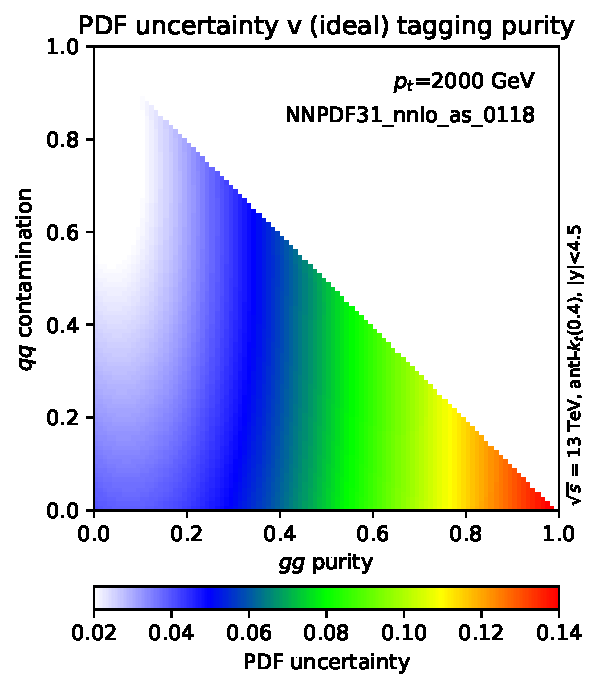
\includegraphics[width=0.42\textwidth, page=1]{figs/performance-plots.pdf} \hfill
\includegraphics[width=0.49\textwidth, page=2]{figs/performance-plots.pdf}
\caption{}
\label{fig:pdf_unc_studies} 
\end{center}
\end{figure}

The next step in our study is to evaluate the current PDF uncertainties, as a function of the final-state flavour composition. 
%
In order to do so, we imagine as a fist step to have at our disposal an idealised tagging procedure that allows us to freely enhance or depress the different partonic components of the final state. We will come back to actual realisations of this tagger later. 
%
In this context, we find useful to define the gluon-gluon ($gg$) purity as
\begin{equation}
gg \, \text{purity}= \frac{\sigma_{gg}}{\sigma_{qq}+\sigma_{qg}+\sigma_{gg}},
\end{equation}
where $\sigma_{ij}$ is the cross section for producing parton $i$ and $j$, evaluated at Born level.  In an analogous way, we can also define the $q q$ contamination is defined analogously, while $q g$ is then fixed by unitarity. Then, for given values $gg$ purity and $qq$ contamination we can evaluate the PDF uncertainty on the cross section.
%
 We decide to perform this estimate using the NNLO PDF set from NNPDF3.1~\cite{Ball:2017nwa} for jets at $2$~TeV.
 %
%The results are shown in Fig.~\ref{fig:pdf_unc_studies}, on the left. 
%
We actually already know from Fig.~\ref{fig:born_studies}, that in the inclusive, i.e.\ untagged, case correspond to $gg$ purity of the order 5\% at $p_t=2$~TeV, while $qq$ and $qg$ makes up roughly 55\% and 40\% of the inclusive sample, respectively. 
%
From the left-hand plot on Fig.~\ref{fig:pdf_unc_studies}, we can then read-off the PDF uncertainty to be of the order of a few percent. This is reflects the fact that the quark parton densities are fairly-well constrained in the region of interest. 
As we move to higher values of the $gg$ purity, the less constrained gluon PDFs start to play a more significant role and, as a consequence, the overall uncertainties goes up. For instance, if we were able to devise a tagger that purifies the $gg$ final state to 80\%, we would increase the PDF uncertainty from 2\% to 12\%. 


\begin{figure}
\begin{center}
\includegraphics[width=0.49\textwidth, page=4]{figs/performance-plots.pdf} \hfill
\includegraphics[width=0.49\textwidth, page=5]{figs/performance-plots.pdf}
\caption{}
\label{fig:performance_studies} 
\end{center}
\end{figure}



\subsection{Conclusion and Outlook}
(Simone)








\subsection*{Acknowledgments}

We thank the participants of Les Houches 2019 for a lively environment and useful discussions.
%%
BN is supported in part by the Office of High Energy Physics of the U.S. Department of Energy under Contract No. DE-AC02-05CH11231.
%
SM is also supported by the curiosity-driven grant "Using jets to challenge the Standard Model of particle physics" from Universit\`a di Genova.

\bibliography{lh2019}

\end{document}
